% !TEX root = ../Thesis.tex
\chapter{Evaluation}

We use the trap-driven simulation framework discussed in the previous chapter to simulate a system with superpage overlays. The workload we use for evaluation is a simulated memory checkpointing system with configurable properties.

For a simple motivational study, the fork-write benchmark is analyzed without simulation using the Linux \verb|perf| tool. Figure \ref{fig:tables} shows the average time and TLB misses for the different configurations of the benchmark, measured by the Linux perf tool. Either a superpage or 512 small pages are allocated, and either one small page or the entire 2MB region is written to in the child process. This benchmark demonstrates the potential for superpage overlays to improve performance. Writing to many 4KB pages is slow due to the high number of TLB misses, but doing copy-on-write with a superpage is slow compared to the 4KB pages when the writes only affect a small amount of memory. Superpage overlays should provide the TLB benefits of superpages while only copying 4KB at a time when the child process writes.
\begin{figure}
    \centering
    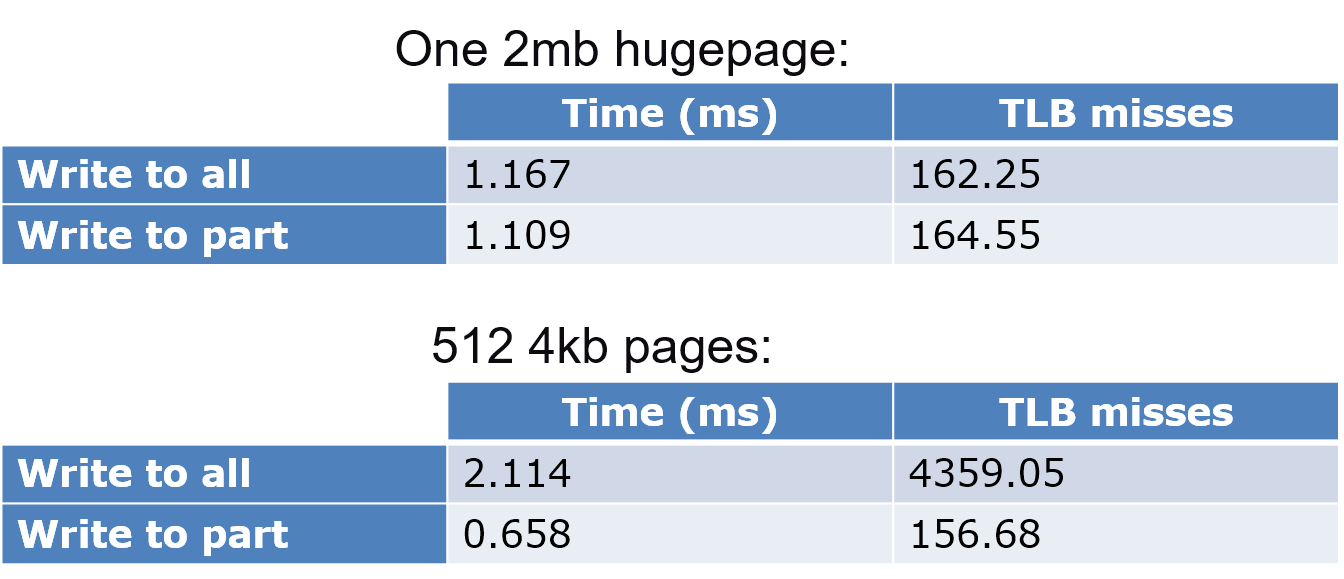
\includegraphics[width=3.2in]{Figures/Table1}
    \caption{Real TLB misses and elapsed time for the 4 different configurations of the fork-write benchmark}
    \label{fig:tables}
\end{figure}

\section{Using Trap-Driven Simulation}

Simulating superpage overlays in the trap-driven framework is fairly simple. We define a \verb|superpage_info| struct that tracks simulation data for every superpage. It includes the virtual and physical address, a flag that is set when the page is marked COW, and the OBitVector. The COW flag is used to identify when the overlay bit should be set for any write to the superpage. When a TLB miss causes a page fault, we can use the information from the page fault and these structs to determine whether to send the address to the simulated 4KB or 2MB TLB for updating. There are 4 possibilities depending on whether the address is a small page or superpage in the real system and whether there is a \verb|superpage_info| struct.

\begin{enumerate}
\item small page fault, no \verb|superpage_info|:
\begin{itemize}
  \item 4KB TLB query
  \item check if superpage coalescing candidate and make \verb|superpage_info| if so
\end{itemize}

\item superpage fault, no \verb|superpage_info|:
\begin{itemize}
  \item 2MB TLB query
  \item create a \verb|superpage_info| and add it to the list
\end{itemize}

\item small page fault, found \verb|superpage_info|:
\begin{itemize}
  \item 2MB TLB query
  \item if physical address not aligned: set overlay bit
  \item if overlay bit set: 4KB TLB query
  \item check if overlay resetting is required and remove \verb|superpage_info| if so
\end{itemize}

\item superpage fault, found \verb|superpage_info|:
\begin{itemize}
  \item 2MB TLB query
  \item if overlay bit set: 4KB TLB query
\end{itemize}
\end{enumerate}

The 4KB and 2MB TLBs being queried are both regular caches with 128 entries and 4-way associativity by default, and the NRU eviction policy discussed in the Trap-Driven Simulation chapter. Every page that is evicted is cleared from the real TLB so that the next access that would miss in the simulated TLB will cause another page fault.

There is also a second simulated TLB that simply models the behavior of a normal system without superpage overlays. It is set up the exact same way, but none of the tests involving \verb|superpage_info| are done. Thus, the superpage overlay system can be compared to a system without overlays with a single benchmark run.

\section{Memory Checkpointing Simulation}

In the Design chapter two forms of memory checkpointing were discussed. Both can be simulated in the same way, since we need not worry about what actually happens to the checkpointed data for the purposes of evaluating superpage overlays. The only difference is that the first type incrementally marks pages writable again as the checkpoint is written out, while the second marks everything writable at once when a commit occurs. We use the first type for this evaluation, though the results would be essentially the same.

The simulation does everything that a real memory checkpointing framework would do, except that the memory snapshots are not actually saved anywhere or used in any way. All writable pages in the address space are marked read-only, and a kernel thread iterates through and waits a small amount of time per page to simulate writing it to nonvolatile memory before clearing the read-only flag and continuing. This checkpoint operation runs once per second.

While the checkpoint is in progress, writes to the pages that are still read-only will be detected and a simulation of COW will occur. If the page is a superpage, there are three different types of COW operation that are compared in this evaluation:

\begin{enumerate}
  \item The superpage is simply copied in whole when a write occurs to any part of it. This is the default COW behavior of Linux.
  \item The superpage is split into small pages and only one 4KB page is copied.
  \item The 4KB segment of the superpage is copied into an overlay.
\end{enumerate}

It is clear that options 2 and 3 will copy the same amount of data. Option 1 will have the fewest TLB misses, since all the memory stays in superpages, while 2 will have the most because all the superpages will soon be split.

The simulation framework is also updated to track the overlays created due to checkpoints separately and implement overlay switching for those pages to limit the number of overlays that exist after many checkpoint iterations. In this way, repeated checkpointing effectively causes superpages to bounce back and forth between two physical memory locations.

\section{Checkpoint Workload}

The last component needed for evaluation is a userspace program to run the checkpoints on. This is just a simple benchmark that simulates a generic memory-intensive workload. The program allocates a large region of memory (which is allocated as superpages via THP), and repeatedly reads or writes random bytes of memory. The percentage of accesses that are writes is configurable, and there is also a locality parameter.

The locality sets the probability distribution of memory access locations. A higher locality means that each access is more likely to be near the previous one. This approximates the behavior of most programs, since in general accesses are likely to cluster around a ``hot'' region. The locality is implemented by setting the probability $p$ of stepping 4KB at a time up or down in memory. A direction is picked randomly, and the program loops, deciding on each iteration whether to take another step or stop based on $p$. Then a read or write is performed at the chosen location based on the write probability.

\section{Goals}

The overall goal of this evaluation is to demonstrate the advantages of using superpage overlays. Memory checkpointing is used as an easy-to-analyze example of a situation that is well suited to overlays, as well as a practical proposal for a tool that becomes much more useful when overlays are enabled. If overlays reduce the impact of checkpoints enough, it may become practical to implement frequent checkpointing in many applications to enable easy error recovery.

Additionally, the memory checkpointing application is a demonstration of the general usefulness of superpage overlays. Any application that heavily relies on COW will behave similarly and get the same benefits. Applications that frequently cause superpages to split will similarly benefit, since any operation that splits a superpage for finer-grained memory management could use overlays to avoid splitting and retain the benefits of superpages.
